\documentclass[conference]{IEEEtran}
\IEEEoverridecommandlockouts
% The preceding line is only needed to identify funding in the first footnote. If that is unneeded, please comment it out.
\usepackage{cite}
\usepackage{amsmath,amssymb,amsfonts}
\usepackage{algorithmic}
\usepackage{graphicx}
\usepackage{textcomp}
\usepackage{xcolor}
\usepackage{multirow}
\usepackage{hyperref}
\usepackage{amsmath,amssymb,amsfonts}
\usepackage{booktabs}
\usepackage{array}
%\usepackage[margin=1in]{geometry}
%\usepackage{mathptmx}
%\usepackage{graphicx}
%\usepackage{listings}
%\usepackage{verbatimbox}
%\usepackage{subfig}
%\usepackage{paralist}
%\usepackage{xspace}
%\usepackage{booktabs}
%\usepackage{color}
%\usepackage{setspace}
%\usepackage{url}
%\usepackage[numbers, sort&compress]{natbib}
%\usepackage{flushend}
%\usepackage{subfig}
%\usepackage{color}
%\usepackage{float}
%\usepackage{amsmath}
%\usepackage{balance}
%\usepackage{amssymb}
%\usepackage{fancybox}
%\usepackage{rotating}
%\usepackage{tablefootnote}
%\usepackage[para,online,flushleft]{threeparttable}
\def\BibTeX{{\rm B\kern-.05em{\sc i\kern-.025em b}\kern-.08em
    T\kern-.1667em\lower.7ex\hbox{E}\kern-.125emX}}
    
    
%\hypersetup{draft}
\begin{document}

\title{A Comparative Analysis of Predicting the Sentiment of Steam Game Reviews Using Deep Neural Networks}




\author{\IEEEauthorblockN{Daniel Lee}
\IEEEauthorblockA{\textit{School of Computing} \\
\textit{Queen's University}\\
Kingston, Canada \\
18dil@queensu.ca}
}

\maketitle

\begin{abstract}
	The gaming industry continues to grow at an alarming rate. Game developers are under increasing pressure to meet the needs of gamers, but do not always knows exactly what gamers want. Game reviews are a method that gamers use to convey their sentiment about the game. For example, negative game reviews can help game developers understand the underlying problems of the game. However, identifying negative reviews can be time consuming as gamers tend to use sarcasm. 
		
	In this paper, we propose a deep learning solution to automatically classify game reviews as either positive or negative. We use 53,764 game reviews from 3,625 Steam games that are labelled from the Steam platform to train a gated recurrent neural network model. We evaluate the performance of the model and compare it against two Naive Bayes classifiers with different resampling strategies; SMOTE and Tomek link, and under-sampling. We find that the deep learning model out-performs the Naive Bayes classifier using SMOTE and Tomek link in all performance metrics, but under-performs compared to the Naive Bayes classifier using under-sampling, with respect to the test accuracy and AUC. However, we do observe that the deep learning model could potentially be improved with more features, tuning, and epochs.
\end{abstract}
\textbf{\textit{Keywords-} Steam; Game reviews; Gated recurrent neural networks; classifier}

\section{Introduction}
\label{sec:intro}
The video game market is growing faster than ever with a projected revenue of approximately \$180 billion in 2021. As the game market continues to evolve, user requirements rapidly increase, making game development more difficult. Game development is becoming more complex and requires a larger team to satisfy the increasing needs of gamers. Thus, it is important for game developers to know how gamers really feel about their games, so game developers can dig deeper into the problems.

One way that game developers can see how gamers feel about their game is through game reviews. Game reviews are an indicator of a gamer's reception towards the game. Prior work~\cite{malavolta2015end} has studied the sentiment of end-users from mobile app reviews. However, game development is vastly different from traditional software development, which could mean that game reviews are likely to be different from traditional mobile app reviews~\cite{pascarella2018video}. 


Furthermore, game reviews may be more susceptible to sarcasm due to the sarcastic culture that Steam is built upon~\cite{baissentiment}. Sarcasm is known to make it difficult for sentiment analysis techniques that use words of the text as indicators of the sentiment~\cite{ganu2009beyond}. As a result, traditional techniques in sentiment analysis are not always accurate, due to the lack of context, sentiment ambiguity, identifying sarcasm, comparatives, regional differences and degree of agreement between humans and machines~\cite{sentimentanalysis}

We believe that traditional sentiment analysis techniques are not well-suited for game reviews. Hence, we want to propose that game developers should use a deep learning approach to better predict the sentiment of gamers. We want to mitigate false-positive results caused by sarcasm as much as possible by learning abstractions of features from the reviews. In short, our intuition is that deep neural networks can learn these complex problems much better than traditional techniques. Although there has been some prior work~\cite{zuo2018sentiment, baissentiment} that utilized traditional sentiment analysis or machine learning techniques to classify game reviews, we purely use a deep learning approach.


%result of the growing game market, user requirements become a subject to change

%The increasing popularity of video games has made game data more available, making games an interesting subject for research. 
% We believe that However, there have only been a few prior empirical studies on games from a software engineering perspective.
%Games are relevant and a growing market.
%Game development is becoming more complex.
%Game developers do not always know how user's perceive their games. 
% End-user perception is important 
% One method of understand the end-user's perception are by analyzing game reviews. 
%Reviews are an important indicator of a gamer's perception of the game.
% Prior work analyzed the reviews of mobile app from the Google Play Store to observe the end-user's perception of the app. In addition, prior research has 

In our paper, we use game reviews from the Steam platform, one of the largest online digital distribution platforms to perform sentiment analysis using a deep learning approach~\cite{lin2019empirical}. In addition, we compare our results to an existing sentiment analysis technique. We conjecture that our deep learning approach will out-perform the sentiment analysis technique, with respect to accuracy and AUC. We want to provide game developers a better approach in classifying game reviews, so they can quickly dive deeper into understanding the gamers needs.
%
%\section{Steam Game Reviews}
%\label{sec:bg}


\section{Related Work}
\label{sec:relatedwork}

\subsection{Sentiment Analysis of Users from Video Game and Mobile App Reviews}


Some prior works have used sentiment analysis techniques on game reviews to classify the gamer's review.


 Str{\aa}{\aa}t and Vergagen~\cite{straaaat2017using} studied the game reviews from \textit{Metacritic.com} to propose an aspect based sentiment analysis to elicit and evaluate user opinions on prior released games. They found that the sentiment of an aspect in a game review impacts its rating. Bais et al.~\cite{baissentiment} used traditional machine learning approaches (i.e., SVM, Logistic Regression, Multinomial Naive Bayes, Turney's unsupervised phrase-labeling algorithm, and a lexicon-based baseline) to classify Steam reviews as positive or negative, finding that SVM with TF-IDF out-performed the others with respect to accuracy, precision, and F1-score after adding hours played and proper weighting of words. Kiran et al.~\cite{kirantwitter} classified positive and negative tweets on the latest review of games using machine learning approaches, and found that maximum entropy has a higher accuracy, precision, and recall than Bayes and SVM. Sirbu et al~\cite{sirbu2016extracting} studied 9,500 game reviews from Amazon and used Principal Component Analysis (PCI) to find five components that could classify game reviews as positive, negative or neutral with a 55\% accuracy. Zuo~\cite{zuo2018sentiment} used Steam game reviews with additional features to train Naive Bayes and Decision Tree classifiers for sentiment analysis on the reviews, finding that the Decision Tree classifier outperformed Naive Bayes with approximately a 75\% accuracy.


Some prior studies have used sentiment analysis techniques on mobile app reviews to understand how the user feels about the app or app features. 


Fu et al.~\cite{fu2013people} studied over 13 million mobile app reviews from the Google Play Store and trained a LDA (i.e. latent dirichlet allocation) model using the negative reviews (1-star or 2-star ratings), and then extracted the topics to observe what users disliked. Liang et al.~\cite{liang2015consumer} used a multifacet sentiment analysis approach on 79 paid and 70 free apps from the iOS app store to explore the relationship between mobile and reviews and the sales, finding that app reviews have a significant influence on the mobile app sales ranking. Sangani and Ananthanarayanan~\cite{sangani2013sentiment} studied the sentiment of mobile app reviews from the iOS App Store by creating topics of interest using WordNet, then ranking the reviews relevant to a topic. They found a number of topics that developers can use to interpret a review, an average rating that displays the general sentiment of a topic, and a representative sample of reviews that provide criticism for a topic. Guzman and Maalej~\cite{guzman2014users} use the NLTK toolkit to extract features from mobile app reviews, then use SentiStrength to assign a sentiment score to the features, and then identified the topics of the reviews. In addition, they calculated the topic sentiment. They proposed an approach to elicit features form mobile app reviews with their corresponding sentiments, which generates two summaries of different scopes that can developers quantify user's feeling about a feature.

In our study, we propose a deep learning approach using a gated recurrent neural network to predict if a Steam game review is positive or negative (i.e., recommended or not recommended) based on the text of the game review.


\subsection{Games Development From a Software Engineering Perspective}

A few prior studies have focused on providing insights for game developers from a software engineering perspective. 

 
Pascarella et al.~\cite{pascarella2018video} studied 60 open source projects to make a comparison between open source game development and traditional open source software development, finding that they are different in various aspects. Politowski et al.~\cite{asurveyonactualsoftwareengineeringprocesses} studied the development of 20 games, finding that at least 30\% of the games still applied a waterfall development paradigm, and 65\% of the games applied iterative practices. Hill et al.~\cite{videogamedevelopmentdifferentfromsoftwaredev} studied 364 survey respondents and 14 interviewees, finding that game developers often avoided automated testing, due to the lack of creativity involved.
	

In our study, we want to help game developers by providing them an accurate approach in classifying game reviews, so they do not waste time on noisy game reviews.


\subsection{Mining Online Game Distribution Platforms}

Several prior studies on mining online distribution platforms focus on Steam. Steam was developed by Valve Corporation and is one of the largest online digital platforms available for PC games~\cite{lin2019empirical}. Steam provides users, who have played the game, the option to leave a \textit{Steam review}\footnote{\url{https://store.steampowered.com/reviews/}} for the game. In addition, the user can label the Steam game review as ``Recommended'' or ``Not Recommended'' (i.e., positive or negative review'). The Steam Community utilizes the``Recommended'' and ``Not Recommended'' ratings to understand the gamer's overall feelings about a game. To the best of our knowledge, there is limited research available on text classification of Steam game reviews.


Sifa et al.~\cite{theplaytimeprinciple} studied the playtime of 6 million users on Steam to discover the fundamental principles of playtime. Lin et al.~\cite{urgentupdates} studied the urgent updates of Steam to observe that developers avoid certain update cycles based on the update pattern. Lin et al.~\cite{lin2017eag} studied the early access model on the Steam, observing that game developers use the early access model to gather early criticisms and positive feedback from newcomers. Lin et al.~\cite{lin2018gr} empirically studied game reviews from Steam, finding that game reviews are different from mobile app reviews. Poretski and Arazy~\cite{placingvalueoncommunitycocreations} empirically studied 45 games from Nexus Mods, finding that user-made game modifications can impact the increase in sales of an original game. Blackburn et al.~\cite{cheatinginonlinegamesasocialnetwork} studied cheaters in the Steam community, observing that the player's network of friends impacted the likelihood of a player becoming a cheater.


In our study, we focus on mining the Steam platform to use sentiment analysis on the game reviews to provide support to game development.


\section{Model}
\label{sec:model}


\begin{figure}[!t]
\center
    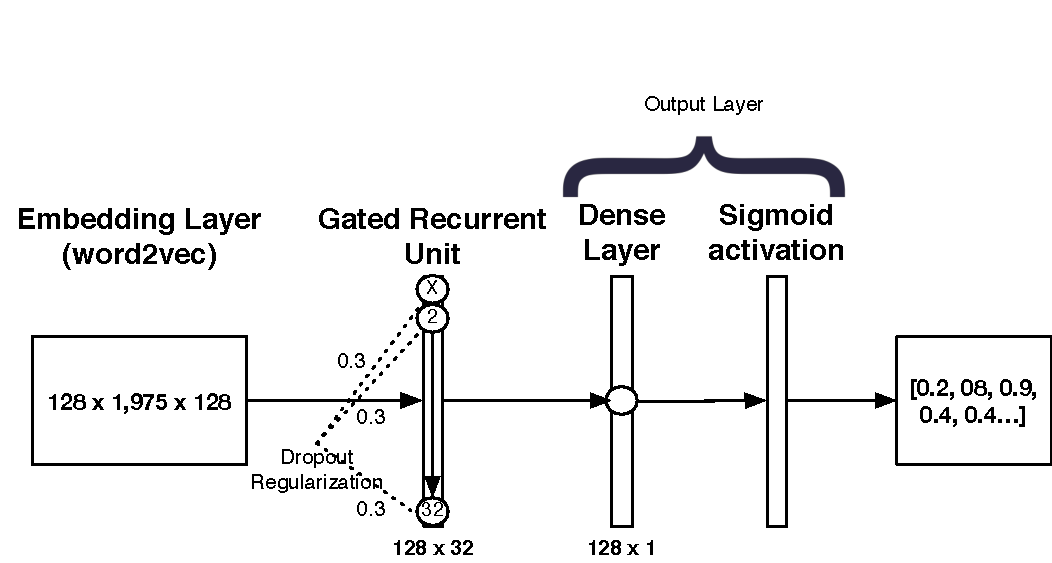
\includegraphics[width=0.5\textwidth]{img/methodology/network_architecture.pdf}
  \caption{The architecture of our gated recurrent neural network.}
  \label{fig:model_architecture}
\end{figure}


In our paper, we will be using a gated recurrent neural network for our deep learning model as it is primarily used for sequential data. Recurrent neural networks have an internal memory state that is capable of remembering prior time steps when propagating through the network. Gated recurrent neural networks are able to out-perform traditional recurrent neural networks in sentiment classification, and perform comparable to long-short term memory networks (i.e., LSTM), while being more computationally efficient~\cite{chung2014empirical, tang2015document}. Figure~\ref{fig:model_architecture} shows an overview of our deep learning network architecture.


Originally, recurrent neural networks had a trouble time remembering long time series data, which led to the vanishing gradient problem. Gated recurrent units (GRU) solve some of the disadvantages of standard recurrent neural networks, such as the vanishing gradient problem with an update and reset gate. The update gate determines how much information from the past propagates to the future and the forget gate determines how much of the past information is forgotten~\cite{updateresetgate, chung2015gated}. 


In the gated recurrent unit, we use dropout and recurrent dropout regularization to prevent overfitting of our data. Dropout regularization assigns a probability on the nodes of a layer, and deactivates the nodes that are exceeding the probability threshold, which allows for more generalization of smaller subsets of information due to the fewer nodes.


To input the Steam game reviews into our recurrent neural network we first develop a Word2vec model to  generate word embeddings. Word embeddings provide contextual vector representations of the words in our Steam game reviews. We pre-train our own Word2vec model using the Steam game reviews. Word2vec utilizes the skip-gram or common bag of words (CBOW) models to create word embeddings. The Skip-gram model produces a probability distribution of the contexts position for each word in the game review~\cite{mikolov2013distributed}. The CBOW model attempts to predict the word based on the context of the word~\cite{ling2015two}. We use the Word2vec algorithm provided by the \textit{Gensim library}\footnote{\url{https://radimrehurek.com/gensim/models/word2vec.html}}. Afterwards, the word embeddings are used in the embedding layer of the neural network. Since, the Word2vec model is pre-trained we do not have to train the embedding layer in each epoch, which saves us some computation time.


The output of our network is a binary classification (``Recommended'' or ``Not Recommended'') of the gamer's sentiment. Thus, we add a final dense layer (i.e., fully connected), with a sigmoid activation function. We use the sigmoid activation function to squeeze the outputs of the gated recurrent unit layer into a value ranging from 0 to 1 because we are performing binary classification. In addition, we use the binary cross-entropy loss function with the Adam optimizer. We use the binary cross-entropy loss function because our task is binary classification. We use the Adam (i.e., adaptive moment estimation) optimizer because it is known to be computationally efficient and uses an adaptive learning rate~\cite{kingma2014adam}.


In addition, we wrapped the entire above-mentioned process in a stratified and shuffled K-fold cross validation to evaluate the model's performance with the data. Due to the time constraint, we only used 5 folds for cross validation. We computed the mean and median accuracy for the training, validation, and test set, along with the mean and median AUC (i.e., area under the curve) for the test set across the folds. Accuracy is defined as:

\[\text{\emph{Accuracy}} = \frac{\text{\emph{TP + TN}}}{\text{\emph{TP + TN + FP +FN}}}\]


TP is the true positive classes; TN is the true negative classes; FP is the false positive classes; FN is the false negative classes. Accuracy can be misleading due to the inherent sensitivity on a given threshold for correctly identified classes. Thus, we also calculated the AUC (i.e area under the curve) because it considers all possible thresholds, whereas the accuracy does not~\cite{ling2003auc}.


Furthermore, we also built two Naive Bayes classifiers to predict the sentiment of Steam game reviews, and used them as baselines in our study. Since, our dataset has a class imbalance, we used two different resampling strategies. Prior work~\cite{batista2003balancing} found that \textit{SMOTE (i.e., synthetic minority oversampling technique) with Tomek links} out-performed \textit{SMOTE over-sampling} with a 91.6\% AUC. Hence, to account for the imbalanced classes in our Steam game reviews, we built one classifier using \textit{SMOTE and Tomek links}, and another classifier using under-sampling.
%We will use a variable-length word vector as my input using the text of Steam game reviews. I explain the general pre-processing steps in Section~\ref{sec:exp}. Thus, I will be using a word embedding network such as \textit{Word2Vec} to generate the word vectors. 

%By using \textit{Python} with the \textit{Keras API}, I will build a 3-layered recurrent neural network (i.e., RNN) with 2 dense layers, and 2 Long-Short Term Memory networks (i.e., LSTM). I chose a recurrent neural network for my text classification problem because it is robust and known to perform well with variable-length text~\cite{zhou2016text,arevian2007recurrent}. Thus, my network architecture will be based on a recurrent neural network.

%Then, I will use 1D max pooling to concatenate the max values from each input group or feature map into a single vector. 
%Furthermore, . More details on the binary classification are in Section~\ref{sec:exp}.


\section{Experiment}
\label{sec:exp}

\begin{figure*}[!t]
\center
    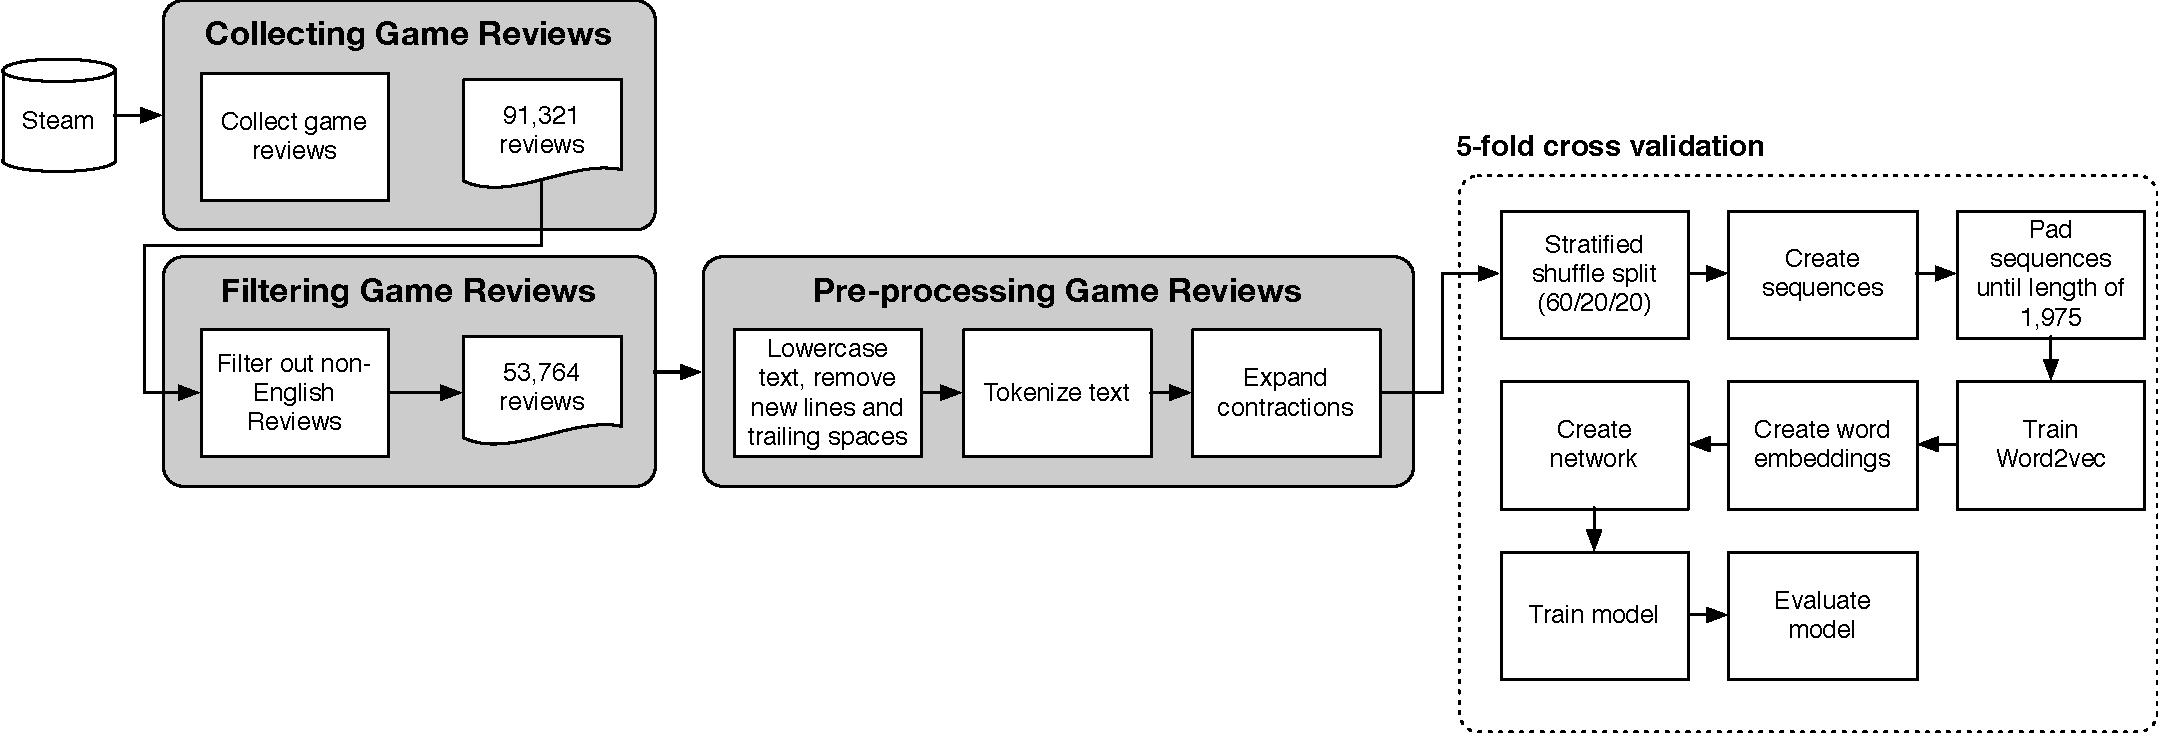
\includegraphics[width=1\textwidth]{img/methodology/dl_method.pdf}
  \caption{An overview of our deep learning methodology.}
  \label{fig:dl_method}
\end{figure*}

In this paper, we used Steam game reviews as the primary dataset. Figure~\ref{fig:dl_method} shows an overview of our experiment. We collected 91,321 Steam game reviews from 4,080 Steam games that are labelled as a 1 or 0 (i.e., ``\textit{Recommended}'' or ``\textit{Not Recommended}''). First, we removed non-English game reviews from our dataset as it could bias our result. We were left with 53,764 Steam game reviews from 3,625 games, which we used for the remainder of our study. Then, we shuffled our dataset and set aside a random sample of 60\% of the dataset as the training set, 20\% as the validation set, and the remaining 20\% as the unseen test set. To prepare the Steam game reviews for the Word2vec model we pre-processed them with the following steps:

\begin{enumerate}
	\item Lowercase text
	\item Remove new lines
	\item Remove trailing white spaces
	\item Tokenization of text
	\item Expand contractions
\end{enumerate}

%Put number of reviews left here
Initially, we used stop-word and punctuation removal in our pre-processing steps, but found that our accuracies dropped. A possible explanation for the drop in accuracies is that stop-words and punctuations emphasize certain parts of the review, which actually help the network learn.


Afterwards, we converted the Steam game review tokens into sequences. We padded the sequences with a number of zeros based on the maximum review length (1,975) across the Steam game reviews. We padded the sequences because the embedding layer in the Keras model requires a fixed input length. Thus, to build and train the deep learning model we used the \textit{Keras library}\footnote{\url{https://keras.io/models/model/}}. The padded sequences of the training and validation sets were used to train the Word2vec model. The Word2vec model was re-trained on each fold.


Furthermore, we noticed a large class imbalance in our Steam game review dataset, where there were almost three times more recommended reviews (1) than not recommended reviews (0). To resolve the class imbalance, we used our class labels to compute a dictionary of class weights with the \textit{Sci-kit learn library}\footnote{\url{https://scikit-learn.org/stable/modules/generated/sklearn.utils.class\_weight.compute\_class\_weight.html}}. Hence, the class weights emphasized the minority class over the majority class. We also tried over-sampling the minority class, but found our deep learning model to perform poorly.


For the hyper-parameters of the gated recurrent network, we used an embedding dimension of 128 for the embedding layer. We tried embedding dimensions of 64 and 100, but found that 128 out-performed them. We started with a dropout regularization probability threshold of 0.2 in the gated recurrent unit layer. Eventually, we ended up using a probability threshold of 0.3 because it performed better than the probability thresholds of 0.2 and 0.4. 


Although the Adam optimizer does not require an initial learning rate, we tried the learning rates 0.01, 0.001 and 0.0001 because prior work has shown significant improvements in performance when using an initial learning rate~\cite{wilson2017marginal}. We decided to use 0.001, as it out-performed the others. For the dense layer, we tried 32 and 64 nodes respectively, but found that 32 nodes out-performed the others

 
 Due to the long runtime of training our network (roughly 650 seconds per epoch), we decided to only run 20 epochs per fold. We also used early stopping with a patience value of 5 to speed up the training of the model. However, we did try patience value of 8 and 10, but did not find a significant difference in prior deep learning models. 
 
 
 Lastly, we compared our deep learning approach with two Naive Bayes classifiers that used different resampling strategies. We assessed all the models based on the accuracy and AUC. In addition, both of the Naive Bayes classifiers used the same data pre-processing steps as our deep learning model. Also, a 5-fold cross validation was used with a stratified shuffle split (80\% training and 20\% test).
 %For the hidden layers, I will use rectified linear units (ReLU) to add non-linearity and try to prevent the vanishing gradient problem.
\section{Results}

In this section, we discuss the results of our models on the Steam game reviews.


\begin{table}[!tp]
\caption{An overview of the results of our deep learning model and two Naive Bayes classifiers.}
\centering
%\resizebox{\textwidth}{!}{
\tabcolsep=0.05cm
\begin{tabular}{lrrr}
\toprule
%\multicolumn{4}{l}{} \\
\begin{tabular}[r]{@{}r@{}}Performance metrics\end{tabular} & \begin{tabular}[r]{@{}r@{}}Gated\\recurrent\\neural\\network model\end{tabular} & \begin{tabular}[r]{@{}r@{}}Naive Bayes \\ classifier with\\ SMOTE and\\Tomek link\end{tabular} &\begin{tabular}[r]{@{}r@{}}Naive Bayes\\ classifier with\\ under-sampling\end{tabular} \\
\midrule
Mean training accuracy & 0.84 &  0.47 & 0.68 \\
Median training accuracy & 0.85 & 0.47 & 0.68\\
\addlinespace
Mean validation accuracy & 0.85 &  - & -\\
Median validation accuracy & 0.85 & - & -\\
\addlinespace
Mean test accuracy & 0.60 & 0.46 & 0.65 \\
Median test accuracy & 0.62 & 0.46 & 0.65\\
\addlinespace
Mean test AUC & 0.59 & 0.51 & 0.65\\
Median test AUC & 0.60 & 0.51 & 0.65\\

\bottomrule
\end{tabular}%}
\label{tab:model_results}
\end{table}

Table~\ref{fig:model_accuracy} shows that our deep learning model from the gated recurrent neural network out-performed the Naive Bayes classifier with SMOTE across all performance metrics. However, we found that our deep learning model was out-performed by the Naive Bayes classifer that used under-sampling based on the performance metrics on the test set. A possible explanation for the poor performance of our deep learning model is that our pre-trained Word2vec model in the 5-fold cross validation model did not capture enough of the gamers vocabulary to generalize onto the test set. Another possible explanation is that we did not train the deep learning model long enough regarding epochs. 

\begin{figure}[!t]
\center
    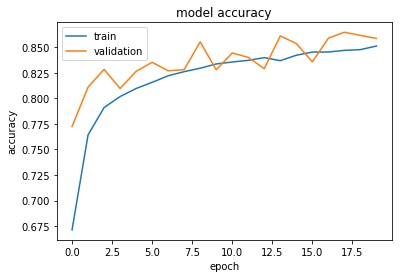
\includegraphics[width=0.5\textwidth]{img/results/model_acc5.png}
  \caption{The deep learning model accuracy per epoch.}
  \label{fig:model_accuracy}
\end{figure}



Figure~\ref{fig:model_accuracy} shows that the training accuracy is still increasing and may need more epochs to converge. In addition, Figure~\ref{fig:model_loss} shows that the training loss is still decreasing and may need more epochs to converge. However, Figure~\ref{fig:model_loss} shows that the model does overfit at certain times, which is shown from the training loss dipping under the validation loss. A possible explanation for the overfitting is because there is a class imbalance, which the class weights may not be fully resolving. It is likely that other measures are required to fix the class imbalance. Based on our results and insights, deep learning-based classifiers for sentiment analysis may not be robust against the inherent slang and sarcasm in game reviews, but does show potential in improving. We believe that more training, tuning, and features can significantly improve our deep learning model's performance.

\begin{figure}[!t]
\center
    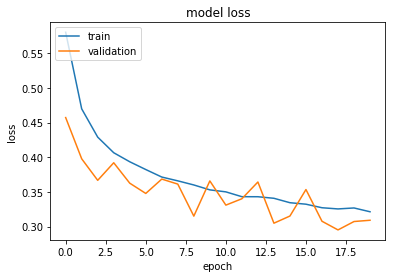
\includegraphics[width=0.5\textwidth]{img/results/model_loss5.png}
  \caption{The deep learning model loss per epoch.}
  \label{fig:model_loss}
\end{figure}

\section{Discussion}
In this section, we discuss some insights regarding the potential for our study, and some criticisms of similar work.

In our paper, we provide an approach of using deep learning to classify the sentiment of Steam game reviews. Although the Naive Bayes classifier out-performed our deep learning model, with respect to the test accuracy and AUC, we believe that adding an auxiliary input like such as hours of gameplay or compensation may help the deep learning model perform better on the test set to combat the sarcasm. For example, a game review may have sarcastic text that portrays the game in the opposite manner, but the hours of gameplay may contradict it. 


To justify using the hours of gameplay as a feature for this problem, we calculated the delta days between the review post date and the initial game release date for just the top 10 games, with respect to the number of Steam game reviews. Figure~\ref{fig:number_of_days} shows the number of days that it took a gamer to post a review after the initial game release. We wanted to see if there was any pattern in how long a gamer played the game before posting reviews based on the median delta days. We observed from Figure~\ref{fig:number_of_days} that there are groups of games where gamers often post the review after the initial game release with a similar median delta days, which means that the hours of gameplay may have an impact on gamers posting a review. Hence, the hours of gameplay may be a significant feature in improving the deep learning model.


Furthermore, our results from Table~\ref{tab:model_results} show that the gated recurrent neural network can learn well based on the training and validation accuracy and loss. However, the training and validation accuracy and loss also reveal that the deep learning model has room for improvement, possibly by increasing the number of epochs.


Bais et al.~\cite{baissentiment} attempted to solve the same problem of classifying the sentiment of Steam game reviews, but using traditional machine learning approaches (e.g., SVM, logistic regression) instead. Although our deep learning model did not out-perform their reported classifier, we believe that the methodology they used has severe flaws that may have biased their results, which we list below:
	\begin{enumerate}
		\item They used a spell corrector to pre-process the Steam game reviews, which may have changed the complete meaning of the sentence or word.
		\item They did not mention handling any class imbalance, which may have biased their accuracy to lean towards the majority class.
		\item They only used 5,000 samples of Steam game reviews, which may have biased the assessment of their classifiers.
	\end{enumerate}
	
  Hence, we believe that the performance of their classifiers would drastically change if they addressed the listed concerns.


	
	\begin{figure}[!t]
\center
    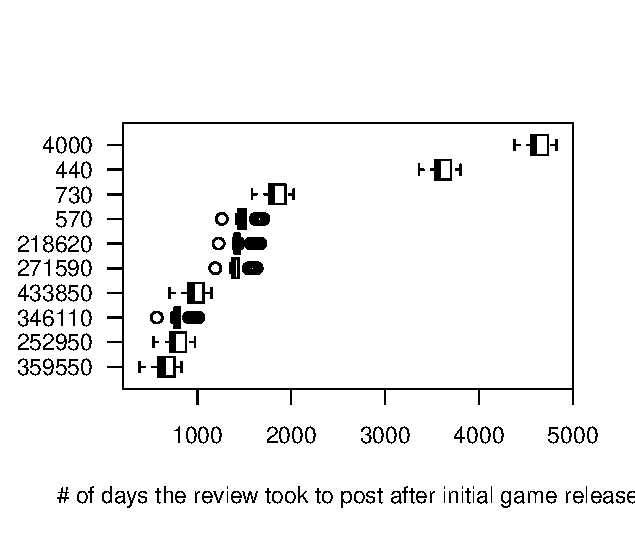
\includegraphics[width=0.46\textwidth]{img/results/boxplot_num_days_after_initial_game_release.pdf}
  \caption{The distribution of the number of days that it took a game review to be posted after the game was initially released per studied game ID.}
  \label{fig:number_of_days}
\end{figure}


\section{Conclusion}

Sentiment analysis of sarcastic text is a challenging problem, even when disregarding external aspects such as context-based sentiment. However, the best solution to this challenging problem could help game developers quickly understand the needs of their gamer base. Hence, we propose a deep learning approach to help game developers accurately classify positive and negative reviews, so they can ultimately save time. We studied 53,764 game reviews from 3,625 Steam games. We built a gated recurrent neural network model, along with two Naive Bayes classifiers with different resampling strategies (i.e., SMOTE and Tomek link, and under-sampling) to account for the class imbalance. 

In result, we found that our deep learning model did train well (85\% median training accuracy and 85\% median validation accuracy), but under-performed against the Naive Bayes classifer that used under-sampling when predicting the unseen test set. On the other hand, we observed that our deep learning model had potential to be improved with more epochs, and possibly with a broader vocabulary and additional features. Hence, there is potential that a deep learning approach can help game developers accurately classify game reviews as positive or negative.
%\balance
\bibliographystyle{IEEEtranS} 
\bibliography{biblio}
%\begin{abstract}
%This document is a model and instructions for \LaTeX.
%This and the IEEEtran.cls file define the components of your paper [title, text, heads, etc.]. *CRITICAL: Do Not Use Symbols, Special Characters, Footnotes, 
%or Math in Paper Title or Abstract.
%\end{abstract}

%\begin{IEEEkeywords}
%component, formatting, style, styling, insert
%\end{IEEEkeywords}

%\section{Introduction}
%This document is a model and instructions for \LaTeX.
%Please observe the conference page limits. 
%
%\section{Ease of Use}
%
%\subsection{Maintaining the Integrity of the Specifications}
%
%The IEEEtran class file is used to format your paper and style the text. All margins, 
%column widths, line spaces, and text fonts are prescribed; please do not 
%alter them. You may note peculiarities. For example, the head margin
%measures proportionately more than is customary. This measurement 
%and others are deliberate, using specifications that anticipate your paper 
%as one part of the entire proceedings, and not as an independent document. 
%Please do not revise any of the current designations.
%
%\section{Prepare Your Paper Before Styling}
%Before you begin to format your paper, first write and save the content as a 
%separate text file. Complete all content and organizational editing before 
%formatting. Please note sections \ref{AA}--\ref{SCM} below for more information on 
%proofreading, spelling and grammar.
%
%Keep your text and graphic files separate until after the text has been 
%formatted and styled. Do not number text heads---{\LaTeX} will do that 
%for you.
%
%\subsection{Abbreviations and Acronyms}\label{AA}
%Define abbreviations and acronyms the first time they are used in the text, 
%even after they have been defined in the abstract. Abbreviations such as 
%IEEE, SI, MKS, CGS, ac, dc, and rms do not have to be defined. Do not use 
%abbreviations in the title or heads unless they are unavoidable.
%
%\subsection{Units}
%\begin{itemize}
%\item Use either SI (MKS) or CGS as primary units. (SI units are encouraged.) English units may be used as secondary units (in parentheses). An exception would be the use of English units as identifiers in trade, such as ``3.5-inch disk drive''.
%\item Avoid combining SI and CGS units, such as current in amperes and magnetic field in oersteds. This often leads to confusion because equations do not balance dimensionally. If you must use mixed units, clearly state the units for each quantity that you use in an equation.
%\item Do not mix complete spellings and abbreviations of units: ``Wb/m\textsuperscript{2}'' or ``webers per square meter'', not ``webers/m\textsuperscript{2}''. Spell out units when they appear in text: ``. . . a few henries'', not ``. . . a few H''.
%\item Use a zero before decimal points: ``0.25'', not ``.25''. Use ``cm\textsuperscript{3}'', not ``cc''.)
%\end{itemize}
%
%\subsection{Equations}
%Number equations consecutively. To make your 
%equations more compact, you may use the solidus (~/~), the exp function, or 
%appropriate exponents. Italicize Roman symbols for quantities and variables, 
%but not Greek symbols. Use a long dash rather than a hyphen for a minus 
%sign. Punctuate equations with commas or periods when they are part of a 
%sentence, as in:
%\begin{equation}
%a+b=\gamma\label{eq}
%\end{equation}
%
%Be sure that the 
%symbols in your equation have been defined before or immediately following 
%the equation. Use ``\eqref{eq}'', not ``Eq.~\eqref{eq}'' or ``equation \eqref{eq}'', except at 
%the beginning of a sentence: ``Equation \eqref{eq} is . . .''
%
%\subsection{\LaTeX-Specific Advice}
%
%Please use ``soft'' (e.g., \verb|\eqref{Eq}|) cross references instead
%of ``hard'' references (e.g., \verb|(1)|). That will make it possible
%to combine sections, add equations, or change the order of figures or
%citations without having to go through the file line by line.
%
%Please don't use the \verb|{eqnarray}| equation environment. Use
%\verb|{align}| or \verb|{IEEEeqnarray}| instead. The \verb|{eqnarray}|
%environment leaves unsightly spaces around relation symbols.
%
%Please note that the \verb|{subequations}| environment in {\LaTeX}
%will increment the main equation counter even when there are no
%equation numbers displayed. If you forget that, you might write an
%article in which the equation numbers skip from (17) to (20), causing
%the copy editors to wonder if you've discovered a new method of
%counting.
%
%{\BibTeX} does not work by magic. It doesn't get the bibliographic
%data from thin air but from .bib files. If you use {\BibTeX} to produce a
%bibliography you must send the .bib files. 
%
%{\LaTeX} can't read your mind. If you assign the same label to a
%subsubsection and a table, you might find that Table I has been cross
%referenced as Table IV-B3. 
%
%{\LaTeX} does not have precognitive abilities. If you put a
%\verb|\label| command before the command that updates the counter it's
%supposed to be using, the label will pick up the last counter to be
%cross referenced instead. In particular, a \verb|\label| command
%should not go before the caption of a figure or a table.
%
%Do not use \verb|\nonumber| inside the \verb|{array}| environment. It
%will not stop equation numbers inside \verb|{array}| (there won't be
%any anyway) and it might stop a wanted equation number in the
%surrounding equation.
%
%\subsection{Some Common Mistakes}\label{SCM}
%\begin{itemize}
%\item The word ``data'' is plural, not singular.
%\item The subscript for the permeability of vacuum $\mu_{0}$, and other common scientific constants, is zero with subscript formatting, not a lowercase letter ``o''.
%\item In American English, commas, semicolons, periods, question and exclamation marks are located within quotation marks only when a complete thought or name is cited, such as a title or full quotation. When quotation marks are used, instead of a bold or italic typeface, to highlight a word or phrase, punctuation should appear outside of the quotation marks. A parenthetical phrase or statement at the end of a sentence is punctuated outside of the closing parenthesis (like this). (A parenthetical sentence is punctuated within the parentheses.)
%\item A graph within a graph is an ``inset'', not an ``insert''. The word alternatively is preferred to the word ``alternately'' (unless you really mean something that alternates).
%\item Do not use the word ``essentially'' to mean ``approximately'' or ``effectively''.
%\item In your paper title, if the words ``that uses'' can accurately replace the word ``using'', capitalize the ``u''; if not, keep using lower-cased.
%\item Be aware of the different meanings of the homophones ``affect'' and ``effect'', ``complement'' and ``compliment'', ``discreet'' and ``discrete'', ``principal'' and ``principle''.
%\item Do not confuse ``imply'' and ``infer''.
%\item The prefix ``non'' is not a word; it should be joined to the word it modifies, usually without a hyphen.
%\item There is no period after the ``et'' in the Latin abbreviation ``et al.''.
%\item The abbreviation ``i.e.'' means ``that is'', and the abbreviation ``e.g.'' means ``for example''.
%\end{itemize}
%An excellent style manual for science writers is \cite{b7}.
%
%\subsection{Authors and Affiliations}
%\textbf{The class file is designed for, but not limited to, six authors.} A 
%minimum of one author is required for all conference articles. Author names 
%should be listed starting from left to right and then moving down to the 
%next line. This is the author sequence that will be used in future citations 
%and by indexing services. Names should not be listed in columns nor group by 
%affiliation. Please keep your affiliations as succinct as possible (for 
%example, do not differentiate among departments of the same organization).
%
%\subsection{Identify the Headings}
%Headings, or heads, are organizational devices that guide the reader through 
%your paper. There are two types: component heads and text heads.
%
%Component heads identify the different components of your paper and are not 
%topically subordinate to each other. Examples include Acknowledgments and 
%References and, for these, the correct style to use is ``Heading 5''. Use 
%``figure caption'' for your Figure captions, and ``table head'' for your 
%table title. Run-in heads, such as ``Abstract'', will require you to apply a 
%style (in this case, italic) in addition to the style provided by the drop 
%down menu to differentiate the head from the text.
%
%Text heads organize the topics on a relational, hierarchical basis. For 
%example, the paper title is the primary text head because all subsequent 
%material relates and elaborates on this one topic. If there are two or more 
%sub-topics, the next level head (uppercase Roman numerals) should be used 
%and, conversely, if there are not at least two sub-topics, then no subheads 
%should be introduced.
%
%\subsection{Figures and Tables}
%\paragraph{Positioning Figures and Tables} Place figures and tables at the top and 
%bottom of columns. Avoid placing them in the middle of columns. Large 
%figures and tables may span across both columns. Figure captions should be 
%below the figures; table heads should appear above the tables. Insert 
%figures and tables after they are cited in the text. Use the abbreviation 
%``Fig.~\ref{fig}'', even at the beginning of a sentence.
%
%\begin{table}[htbp]
%\caption{Table Type Styles}
%\begin{center}
%\begin{tabular}{|c|c|c|c|}
%\hline
%\textbf{Table}&\multicolumn{3}{|c|}{\textbf{Table Column Head}} \\
%\cline{2-4} 
%\textbf{Head} & \textbf{\textit{Table column subhead}}& \textbf{\textit{Subhead}}& \textbf{\textit{Subhead}} \\
%\hline
%copy& More table copy$^{\mathrm{a}}$& &  \\
%\hline
%\multicolumn{4}{l}{$^{\mathrm{a}}$Sample of a Table footnote.}
%\end{tabular}
%\label{tab1}
%\end{center}
%\end{table}
%
%\begin{figure}[htbp]
%\centerline{\includegraphics{fig1.png}}
%\caption{Example of a figure caption.}
%\label{fig}
%\end{figure}
%
%Figure Labels: Use 8 point Times New Roman for Figure labels. Use words 
%rather than symbols or abbreviations when writing Figure axis labels to 
%avoid confusing the reader. As an example, write the quantity 
%``Magnetization'', or ``Magnetization, M'', not just ``M''. If including 
%units in the label, present them within parentheses. Do not label axes only 
%with units. In the example, write ``Magnetization (A/m)'' or ``Magnetization 
%\{A[m(1)]\}'', not just ``A/m''. Do not label axes with a ratio of 
%quantities and units. For example, write ``Temperature (K)'', not 
%``Temperature/K''.
%
%\section*{Acknowledgment}
%
%The preferred spelling of the word ``acknowledgment'' in America is without 
%an ``e'' after the ``g''. Avoid the stilted expression ``one of us (R. B. 
%G.) thanks $\ldots$''. Instead, try ``R. B. G. thanks$\ldots$''. Put sponsor 
%acknowledgments in the unnumbered footnote on the first page.

%\section*{References}
%
%Please number citations consecutively within brackets \cite{b1}. The 
%sentence punctuation follows the bracket \cite{b2}. Refer simply to the reference 
%number, as in \cite{b3}---do not use ``Ref. \cite{b3}'' or ``reference \cite{b3}'' except at 
%the beginning of a sentence: ``Reference \cite{b3} was the first $\ldots$''
%
%Number footnotes separately in superscripts. Place the actual footnote at 
%the bottom of the column in which it was cited. Do not put footnotes in the 
%abstract or reference list. Use letters for table footnotes.
%
%Unless there are six authors or more give all authors' names; do not use 
%``et al.''. Papers that have not been published, even if they have been 
%submitted for publication, should be cited as ``unpublished'' \cite{b4}. Papers 
%that have been accepted for publication should be cited as ``in press'' \cite{b5}. 
%Capitalize only the first word in a paper title, except for proper nouns and 
%element symbols.
%
%For papers published in translation journals, please give the English 
%citation first, followed by the original foreign-language citation \cite{b6}.
%
%\begin{thebibliography}{00}
%\bibitem{b1} G. Eason, B. Noble, and I. N. Sneddon, ``On certain integrals of Lipschitz-Hankel type involving products of Bessel functions,'' Phil. Trans. Roy. Soc. London, vol. A247, pp. 529--551, April 1955.
%\bibitem{b2} J. Clerk Maxwell, A Treatise on Electricity and Magnetism, 3rd ed., vol. 2. Oxford: Clarendon, 1892, pp.68--73.
%\bibitem{b3} I. S. Jacobs and C. P. Bean, ``Fine particles, thin films and exchange anisotropy,'' in Magnetism, vol. III, G. T. Rado and H. Suhl, Eds. New York: Academic, 1963, pp. 271--350.
%\bibitem{b4} K. Elissa, ``Title of paper if known,'' unpublished.
%\bibitem{b5} R. Nicole, ``Title of paper with only first word capitalized,'' J. Name Stand. Abbrev., in press.
%\bibitem{b6} Y. Yorozu, M. Hirano, K. Oka, and Y. Tagawa, ``Electron spectroscopy studies on magneto-optical media and plastic substrate interface,'' IEEE Transl. J. Magn. Japan, vol. 2, pp. 740--741, August 1987 [Digests 9th Annual Conf. Magnetics Japan, p. 301, 1982].
%\bibitem{b7} M. Young, The Technical Writer's Handbook. Mill Valley, CA: University Science, 1989.
%\end{thebibliography}
%\vspace{12pt}
%\color{red}
%IEEE conference templates contain guidance text for composing and formatting conference papers. Please ensure that all template text is removed from your conference paper prior to submission to the conference. Failure to remove the template text from your paper may result in your paper not being published.
% BibTeX users please use one of


\end{document}
